\subsection{Dijets of light and heavy flavors}


\begin{figure}[h]
\begin{center}
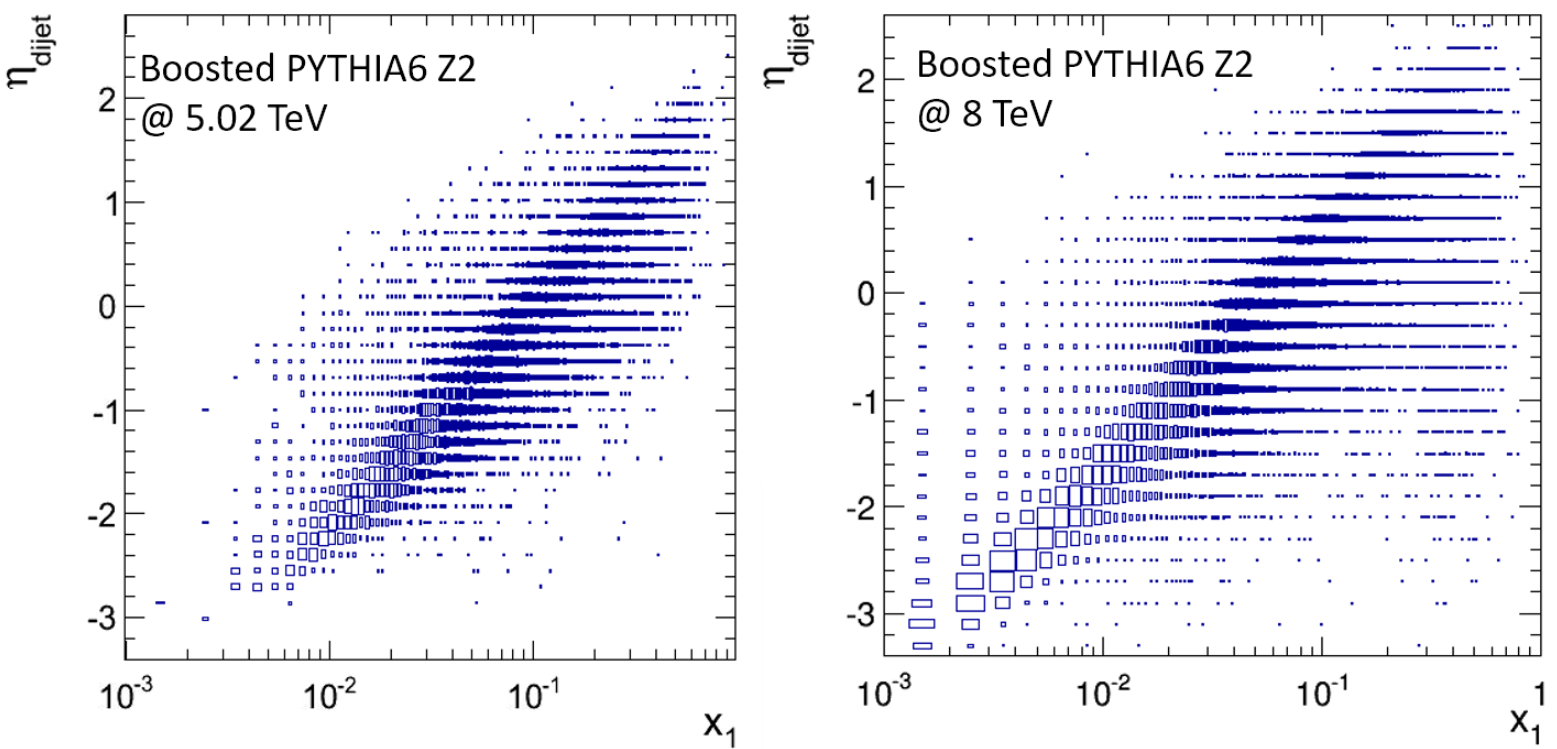
\includegraphics[width= 0.9\textwidth]{figures/x_vs_eta.png}
\caption{Correlations between dijet $\eta_{\rm dijet} = \eta_{1} + \eta_{2}$ 
and parton Bjorken-$x$ from Pb nuclei at \rootsNN\ = 5.02 TeV 
(left) and 8.16 TeV (right) from the boosted {\sc pythia} event generator.}
\label{fig:dijetCorr}
\end{center}
\end{figure}

The measurement of dijet pseudorapidity distributions were 
shown to be sensitive to nPDF effects~\cite{Paukkunen:2014pha}.
Earlier CMS measurement in pPb collisions at \rootsNN\ = 5.02 TeV
has been used to discriminate between different nPDF sets~\cite{Chatrchyan:2014hqa}. 
The tight correlation shown in Fig.~\ref{fig:dijetCorr} between 
dijet $\eta_{\rm dijet} = \eta_{1} + \eta_{2}$ and parton $x$ from Pb nuclei
is the underlying reason of the sensitivity to nPDF. At \rootsNN\ = 8.16 TeV, 
the slope of the correlation varies as $x \approx 1/\sqrt{s_{\rm NN}}$. 
This allows us to push toward a wider $x$ coverage at higher collision energy
within the same detector acceptance. Moreover, with the increase in 
di-b-jet cross section at \rootsNN\ = 8.16 TeV. It will be possible to perform 
the measurement of $\eta_{\rm dijet}$ distributions where both 
leading and subleading jets are tagged as b-jets. As 96\% of 
di-b-jet production is from gluon fusion processes, such a measurement
will be a clean probe of gluon nPDF.


\begin{figure}[h]
\begin{center}
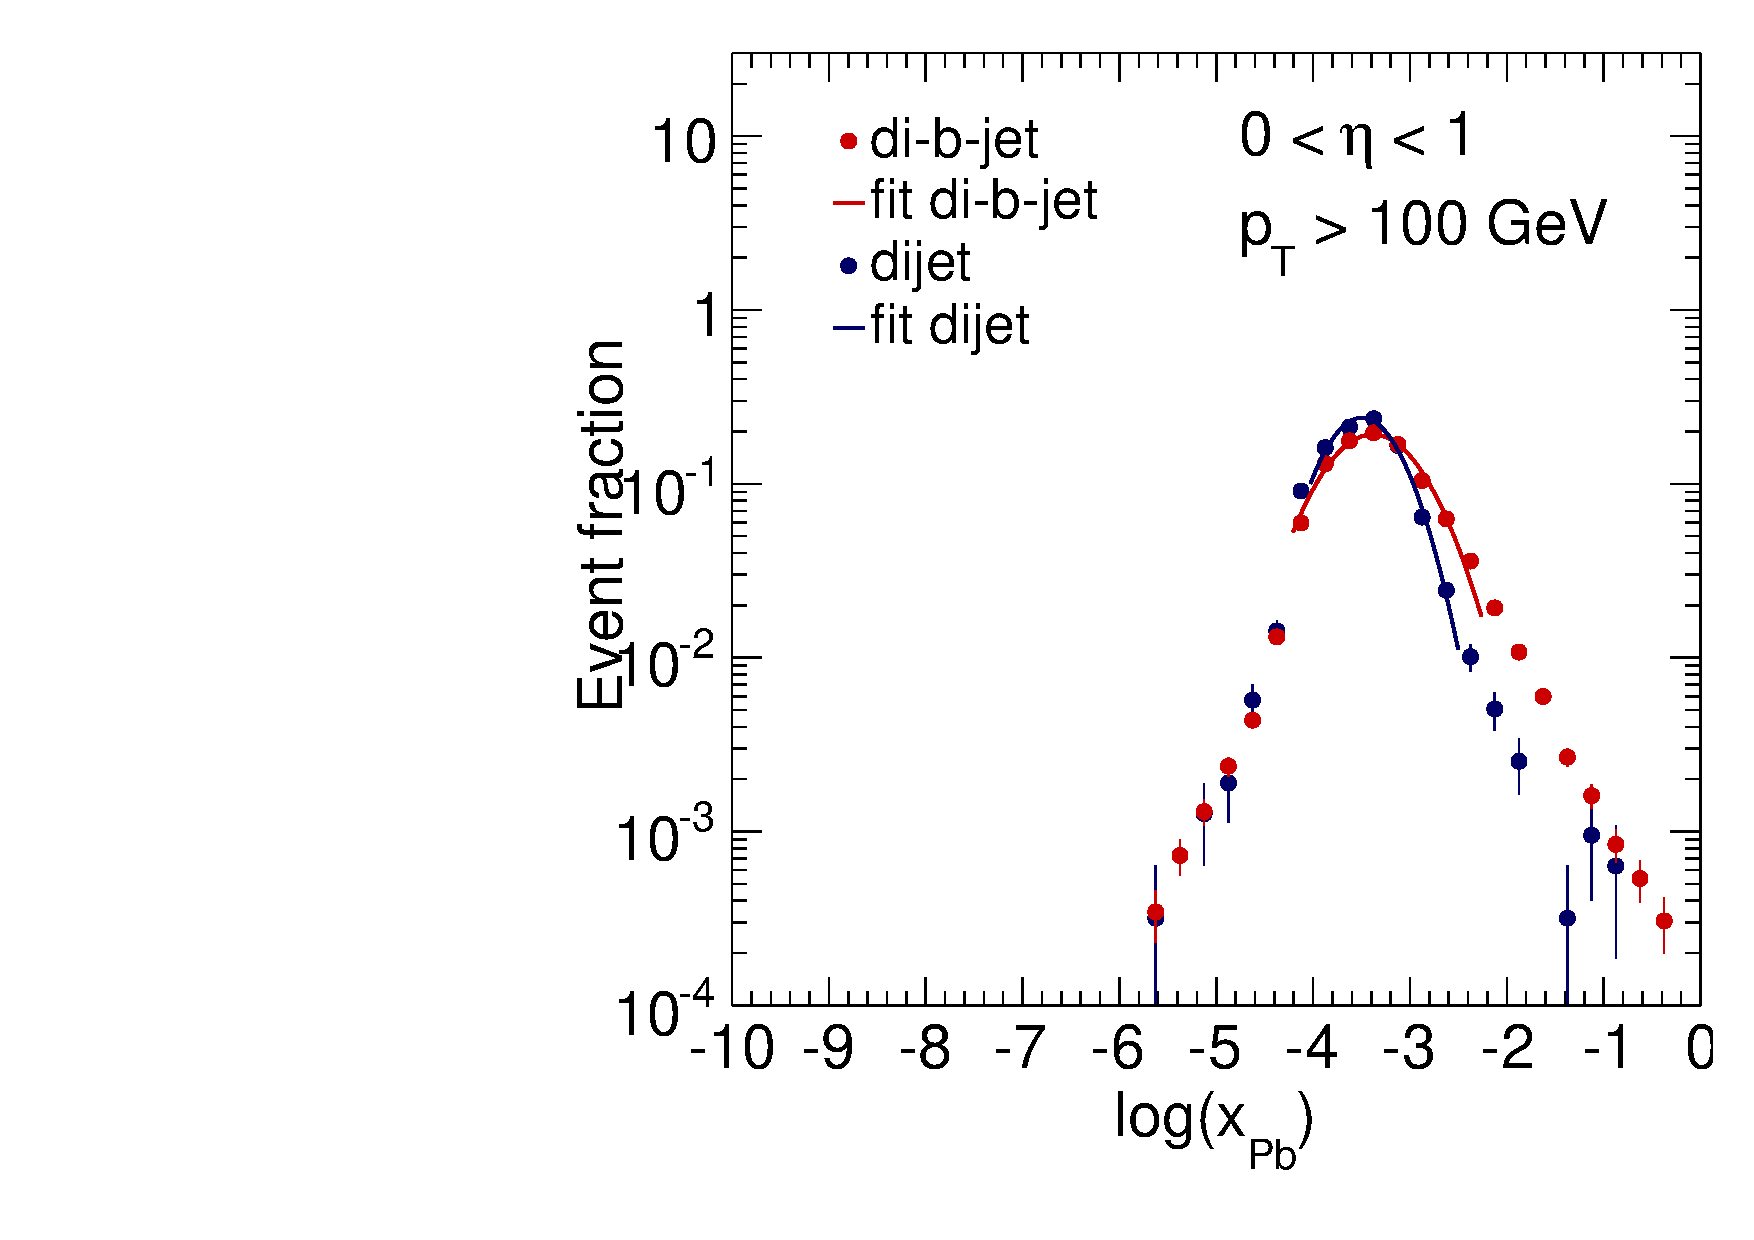
\includegraphics[width= 0.4\textwidth]{figures/DistCompareBJetInclusive.pdf}
\caption{ Distribution of $x_{\rm Pb}$ in log scale for $0<\eta_{\rm dijet}<1$
and $\pt^{\rm ave} > 100$ GeV/c in boosted {\sc pythia} event generator.}
\label{fig:distX}
\end{center}
\end{figure}

Different $x$ values can be probed by selecting on $\eta_{\rm dijet}$, 
while different $Q$ values can be chosen by posing requirements 
on the average \pt\ of the dijets $\pt^{\rm ave} = (p_{\rm T,1} + p_{\rm T,2})/2$.
The expected $x$--$Q$ coverage is calculated by parametrizing 
the $x_{\rm Pb}$ distributions in boosted {\sc pythia} event generator
for a specific $\eta_{\rm dijet}$ and $\pt^{\rm ave}$ selections. 
An example case is shown in Fig.~\ref{fig:distX}. To get a cleaner
estimate of dijet contributions, Gaussian fits are performed 
to exclude the long tails on both sides of the distribution, which are 
potentially contaminated by 3-jet events. The region of the Gaussian
curves outside a certain winder around the mean is scaled
according to the expected integrated luminosity. The region of sensitivity is determined 
by when the number of events outside of this region on either side of 
the mean, given as $0.5 \times {\rm ErfcInverse}((x-\mu)/(\sqrt{2}\sigma))$, 
falls below $1/\epsilon_{\rm stat}^{2}$. The same procedure is also applied 
in deriving the sensitive region of $Q$. The reach in $x$ and $Q$ values 
are calculated in several bins of $\eta_{\rm dijet}$ and $\pt^{\rm ave}$ 
and overlaid as patches of areas on the $x$--$Q$ plane. The results are shown 
in Figs.~\ref{fig:xQscanBjet} for di-b-jets and \ref{fig:xQscanInclusive} 
for inclusive dijets, respectively.


\begin{figure}[h]
\begin{center}
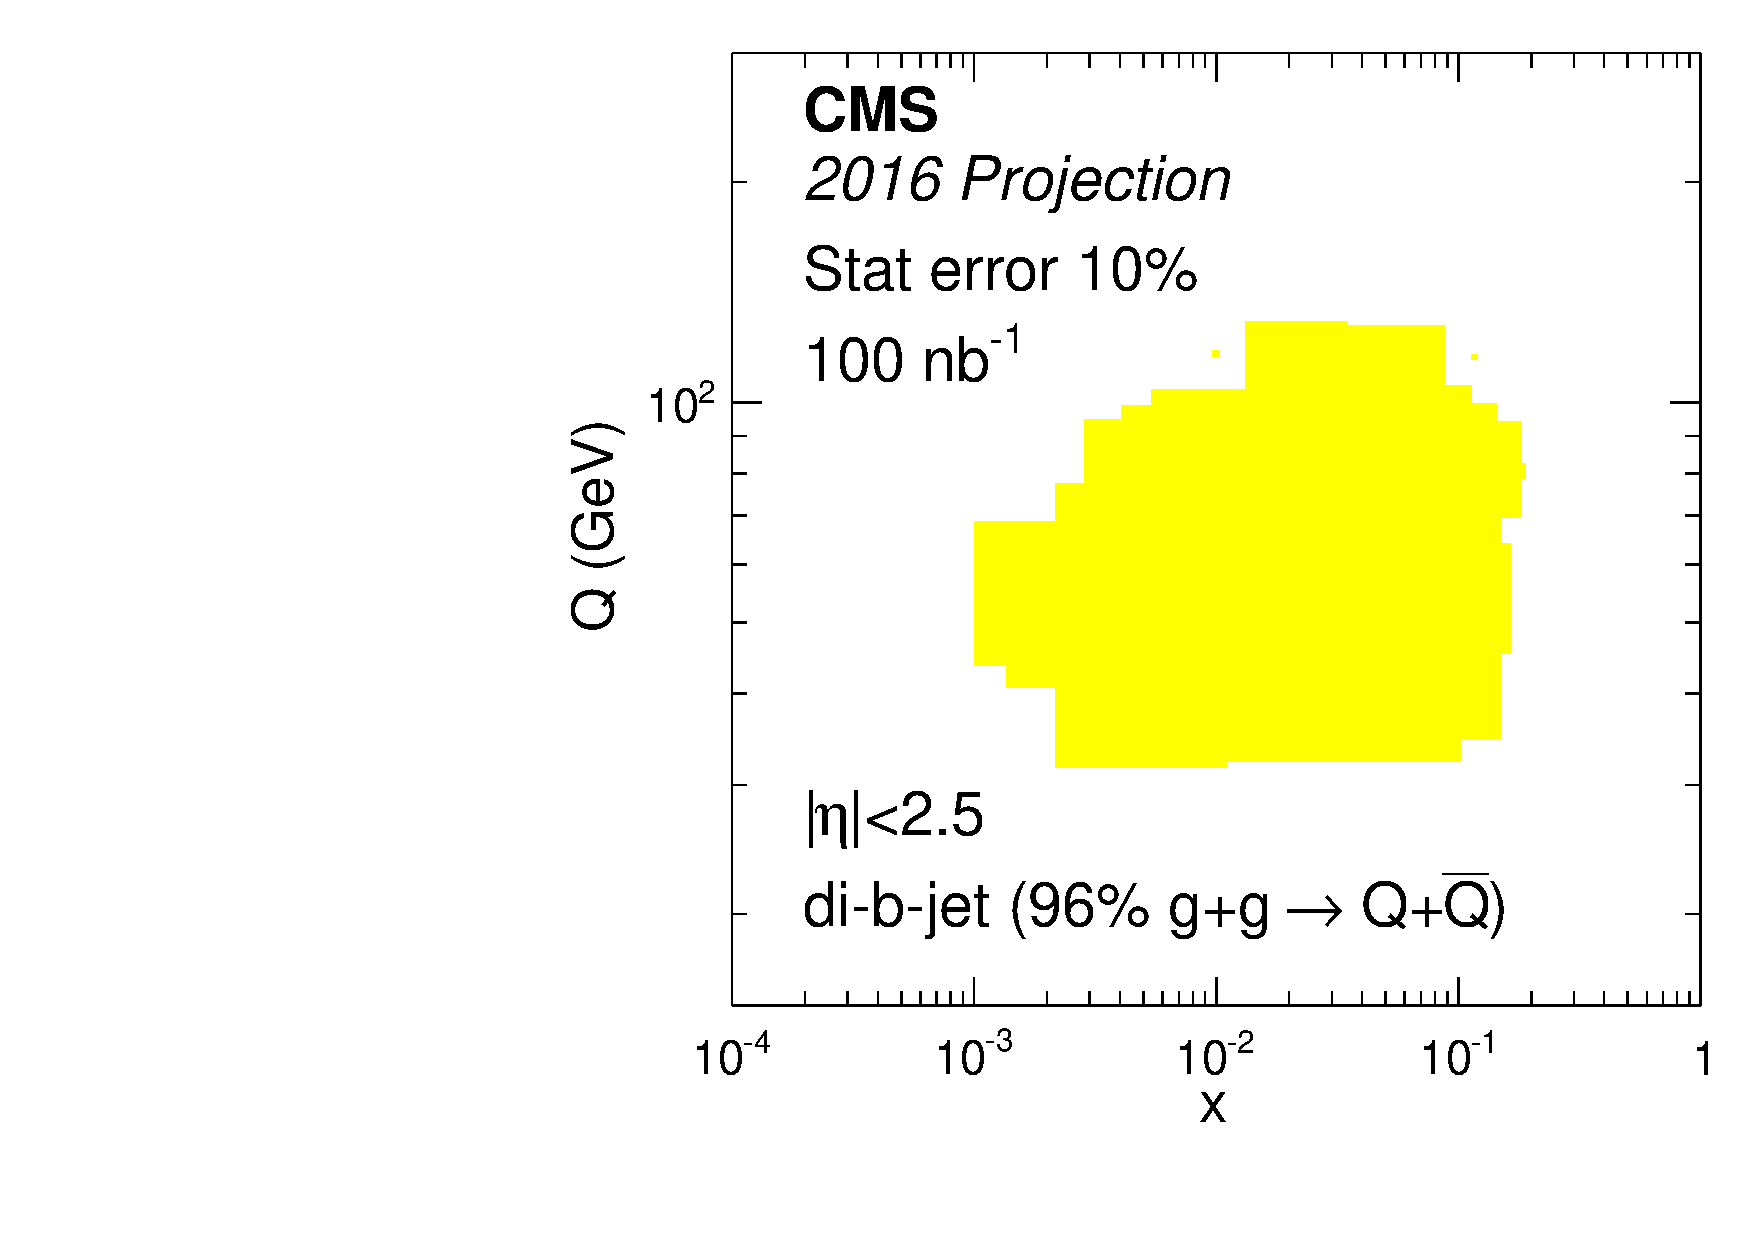
\includegraphics[width= 0.47\textwidth]{figures/filledQX_Lumi100_BJet.pdf}
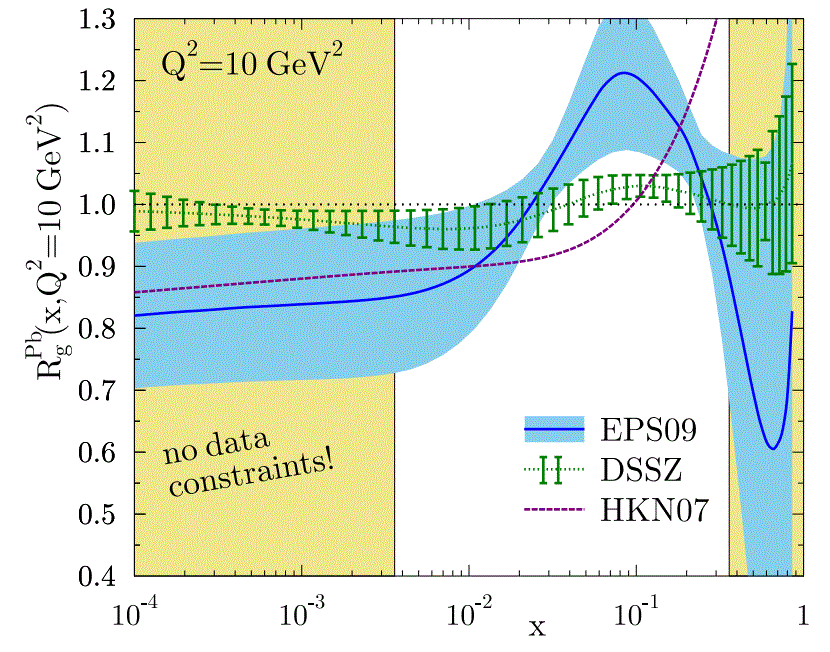
\includegraphics[width= 0.47\textwidth]{figures/eps09_10GeV_Gluon_nPDF.png}
\caption{Left: The $x$--$Q$ scan plot for di-b-jet processes 
with an integrated luminosity of 100 nb$^{-1}$ for pPb collisions
at \rootsNN\ = 8.16 TeV. Right: The gluon nuclear modification factors 
for the lead nucleus at $Q^{2}$ = 10 GeV$^{2}$.}
\label{fig:xQscanBjet}
\end{center}
\end{figure}

Assuming an integrated luminosity of 100 nb$^{-1}$ for pPb collisions
at \rootsNN\ = 8.16 TeV, the resulting $x$--$Q$ scan plot for di-b-jet processes 
is shown in Fig.~\ref{fig:xQscanBjet} (left). As one can see, a high-luminosity
pPb run in 2016 will provide constraints to nPDF in small-$x$ region down to
$3-4 \times 10^{-3}$. In this $x$ regime, there are no existing data
constraints to the gluon nPDF, as shown in Fig.~\ref{fig:xQscanBjet} (right)~\cite{Paukkunen:2014nqa}.

\begin{figure}[h]
\begin{center}
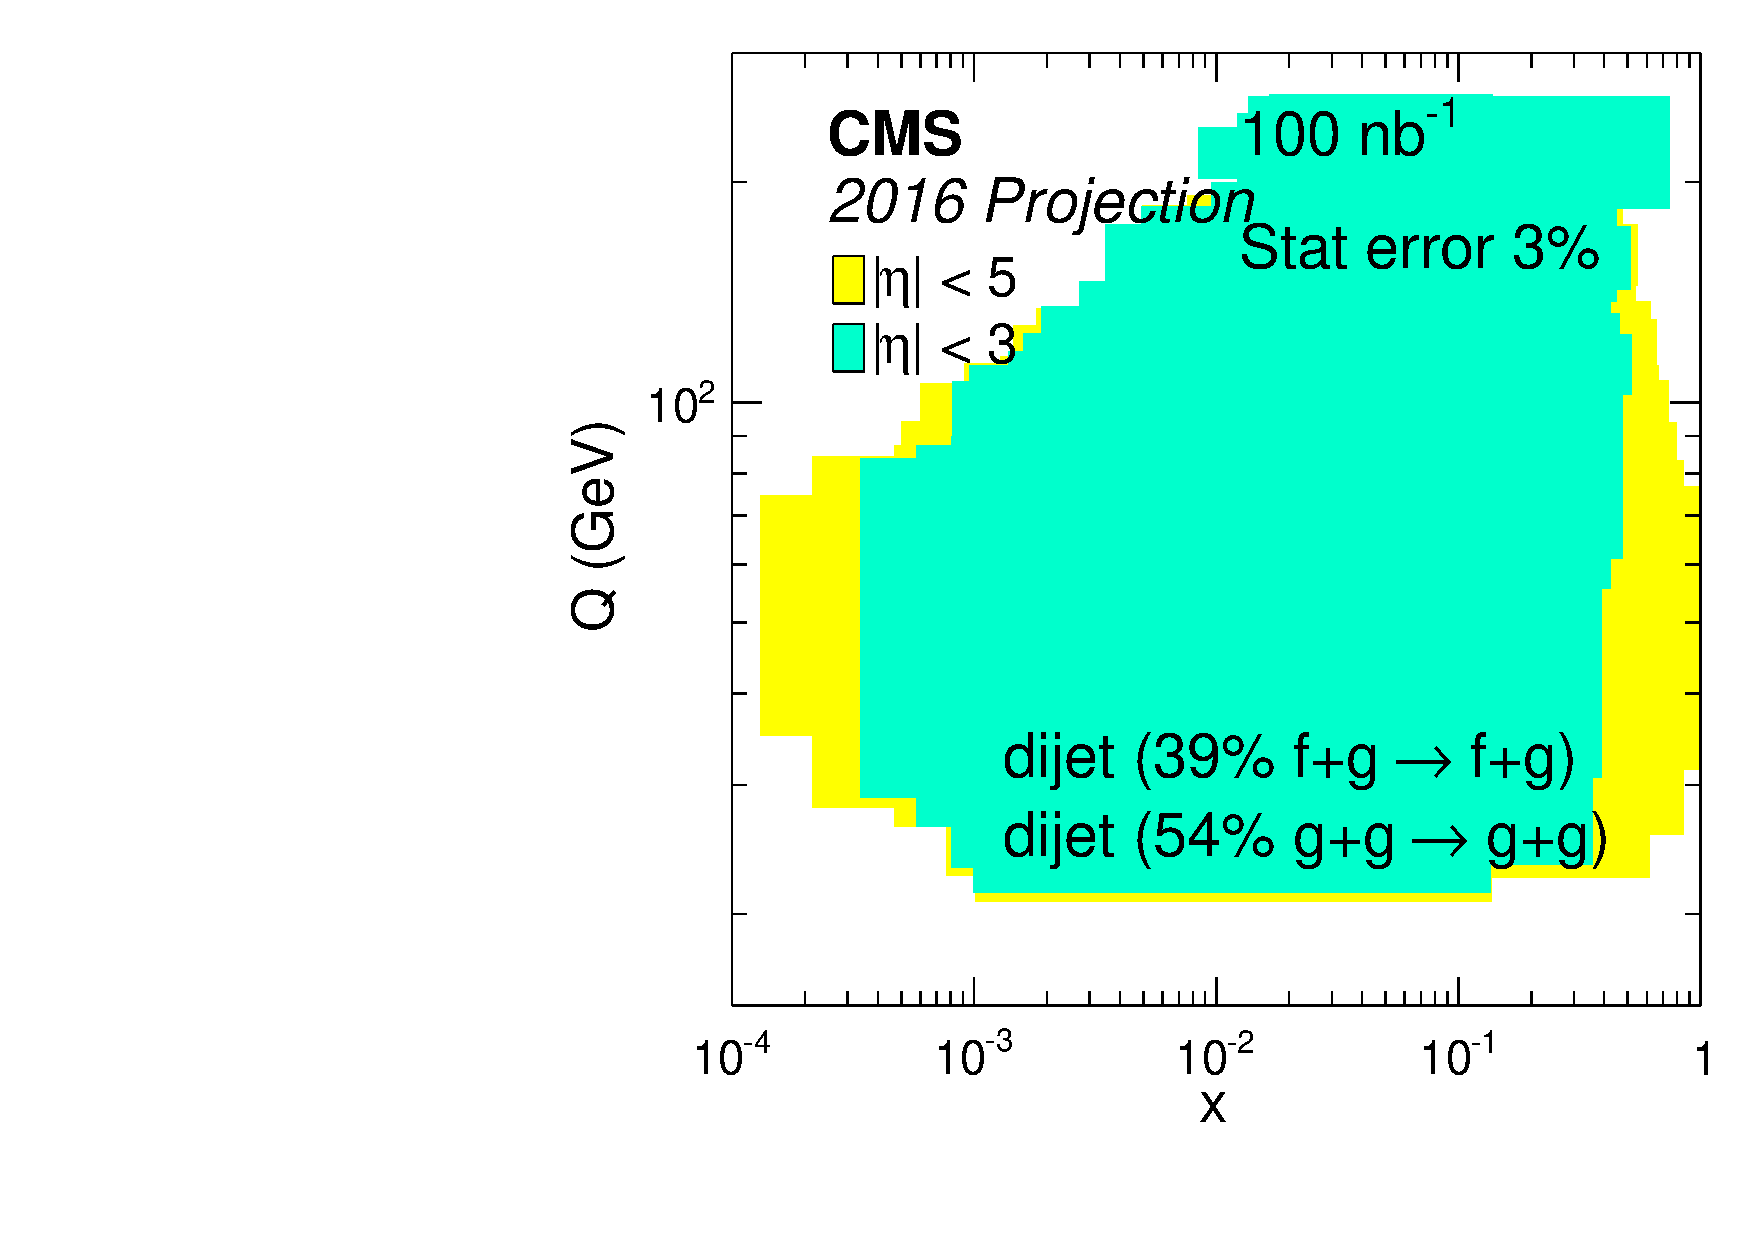
\includegraphics[width= 0.5\textwidth]{figures/filledQX_Lumi100_InclusiveJet_etaComparison.pdf}
\caption{The $x$--$Q$ span of inclusive dijet measurement for the two pseudorapidity selections 
for a measurement with better than $3\%$ statistical precision. }
\label{fig:xQscanInclusive}
\end{center}
\end{figure}


For inclusive flavor dijets, there are significant contributions
from $f + g \rightarrow f + g$ ($39 \%$) processes in addition to gluon fusion 
($54 \%$) processes.Therefore, they do not provide a clean handle on 
the gluon nPDF, which is much less constrained comparing to quark nPDF.
However, due to an abundance of inclusive dijets produced in the collisions,
they can be used to probe a much wider $x$--$Q$ range. The $x$ reach of b-jet measurement 
is limited by the $\eta$ coverage of the tracker, i.e. $|\eta| < 2.5$. 
However, the untagged flavor jet measurements can be extended up to 
$\eta = 3$ with good control on systematic uncertainties and up to $\eta = 5$ if the total 
integrated luminosity is sufficient to allow one to calibrate the energy response of 
Hadronic Forward (HF) calorimeters. The $x$--$Q$ span of inclusive dijet 
measurement is shown in Fig.~\ref{fig:xQscanInclusive} for the two pseudorapidity selections 
for a measurement with better than $3\%$ statistical precision. 
The statistical uncertainty as a function of $x$ in the high-$x$ region 
is shown in Fig.~\ref{fig:XreachWithPseudorapidity} for different 
luminosity scenarios, 10, 25, 50 and 100 nb$^{-1}$, for $|\eta| < 3$ (left) 
and for $|\eta| < 5$ (right). For dijets selected 
within $|\eta| < 3$, where systematic uncertainties are well under control, 
the reach in large-$x$ regime clearly benefits from a high-luminosity pPb run. 
With an integrated luminosity of 100 nb$^{-1}$, it is possible to measure up to $x = 0.6$ 
within $10 \%$ statistical accuracy.

\begin{figure}[h]
\begin{center}
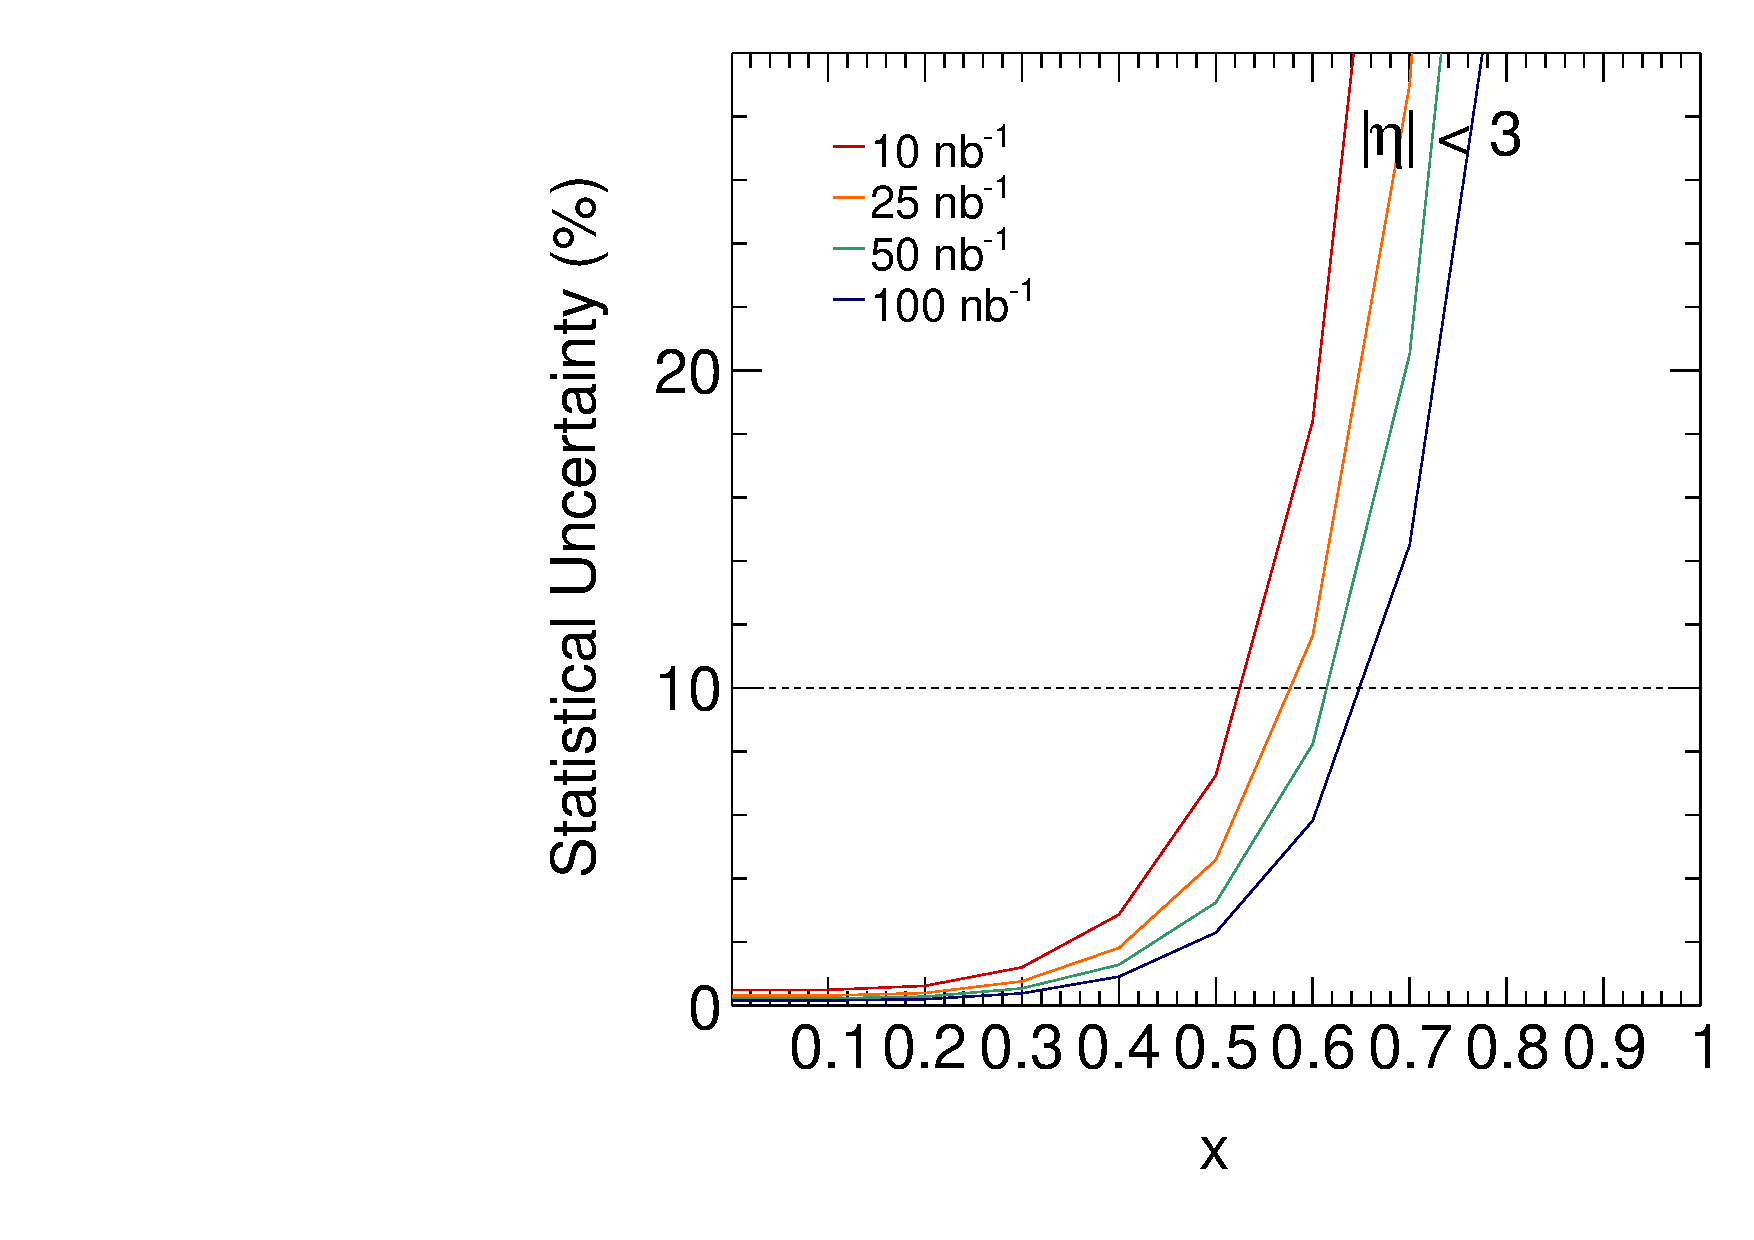
\includegraphics[width= 0.4\textwidth]{figures/xStat_eta3_inclusiveJet.pdf}
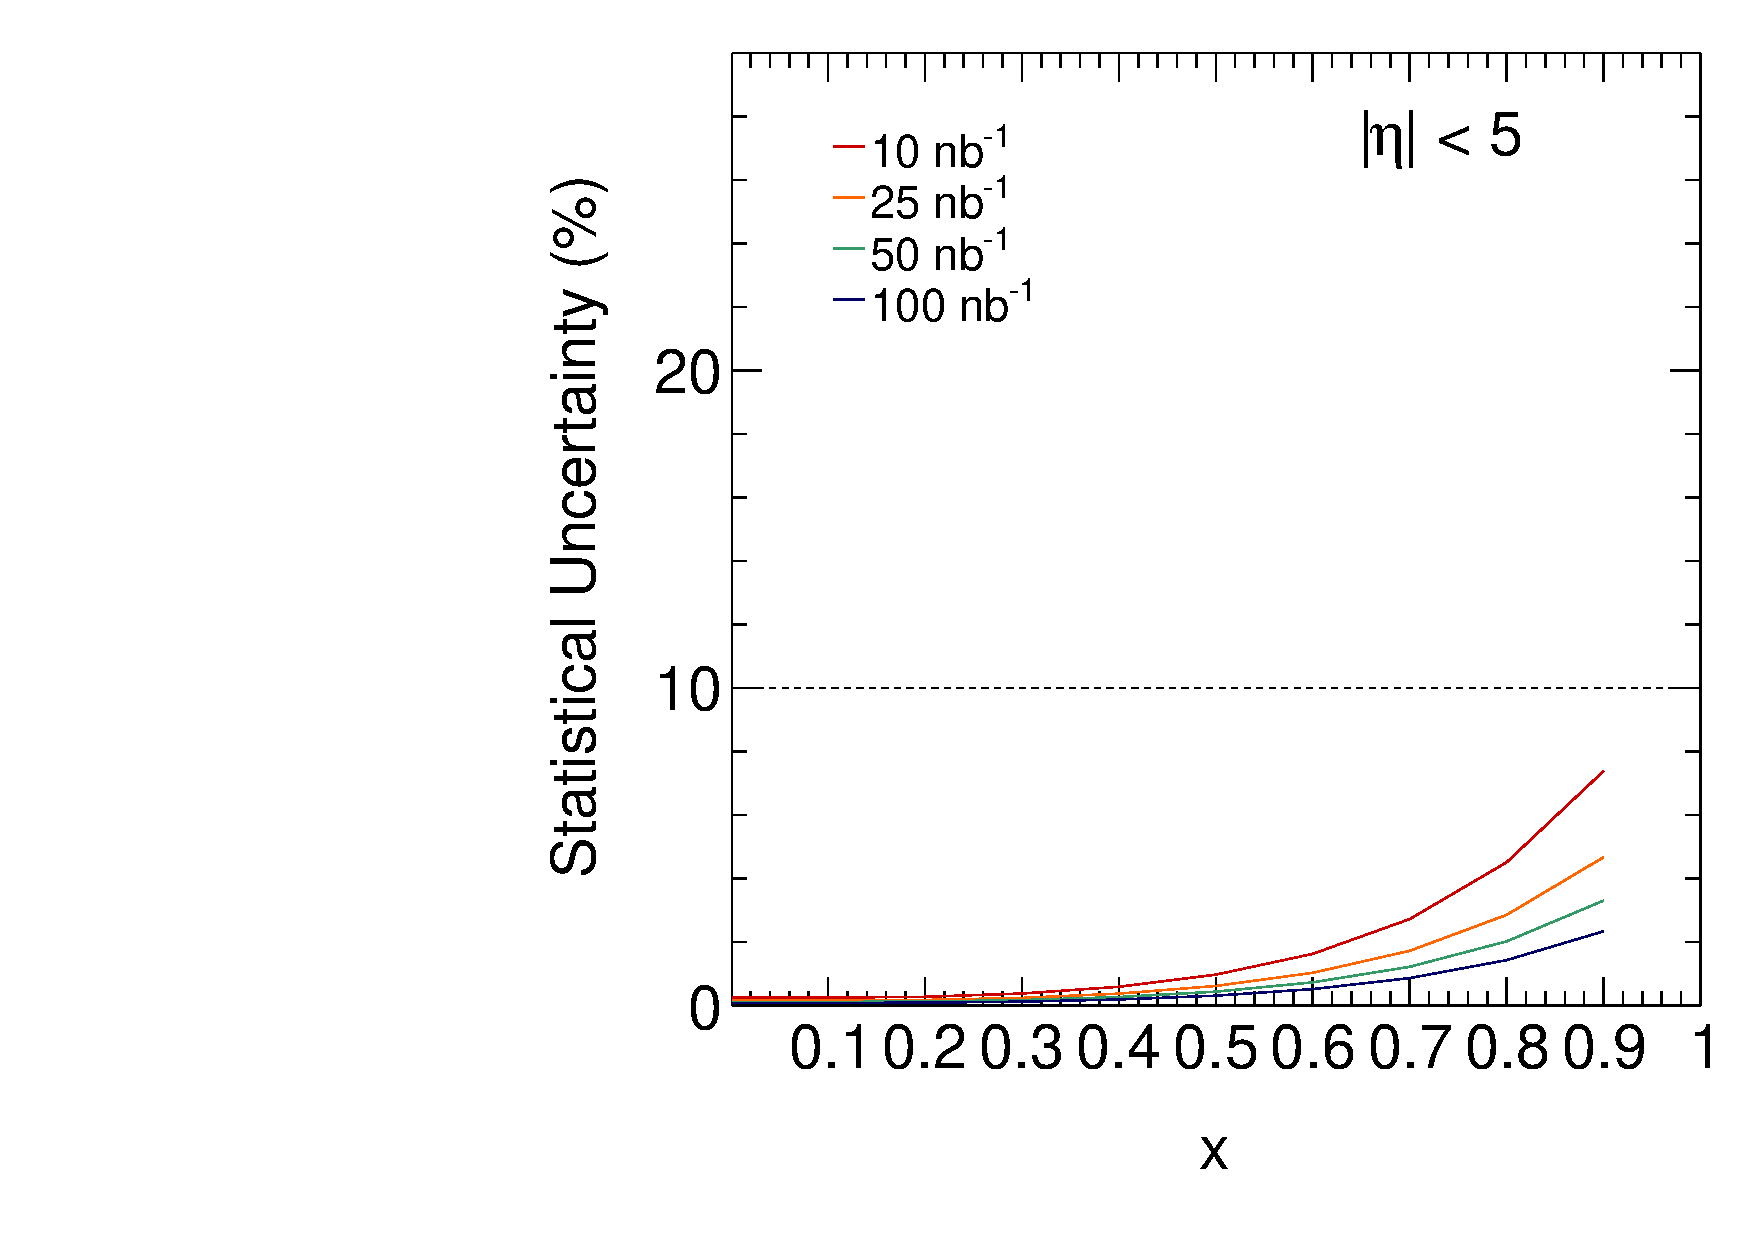
\includegraphics[width= 0.4\textwidth]{figures/xStat_eta5_inclusiveJet.pdf}
\caption{The projected statistical uncertainty as a function of $x$ in the high-$x$ region 
for different luminosity scenarios of L$_{\rm int}$ = 10, 25, 50 and 100 nb$^{-1}$, 
for $|\eta| < 3$ (left) and for $|\eta| < 5$ (right).}
\label{fig:XreachWithPseudorapidity}
\end{center}
\end{figure}

For $|\eta| < 5$ selection, the statistical uncertainty becomes negligible
and is no longer the dominant factor on the precision of the measurement. 
Systematic uncertainties caused by the jet energy scale uncertainties in HF 
become more significant. With increased integrated luminosity, the systematic 
uncertainties can also be reduced by applying data-driven methods to calibrate HF.
This has been demonstrated in pp data at \roots\ = 7 and 8 TeV, as shown in 
Fig.~\ref{fig:jetJES}. Even with L$_{\rm int}$ = $36$ pb$^{-1}$ pp data sample, 
the uncertainty on corrections in HF is $\approx 10 \%$. These uncertainties shrink 
to only $4\%$ with an integrated luminosity of $20$ fb$^{-1}$. Therefore, it will 
only be possible to probe high-$x$ values that are sensitive to a very 
interesting range of nPDF modifications with high luminosity data.

\begin{figure}[h]
\begin{center}
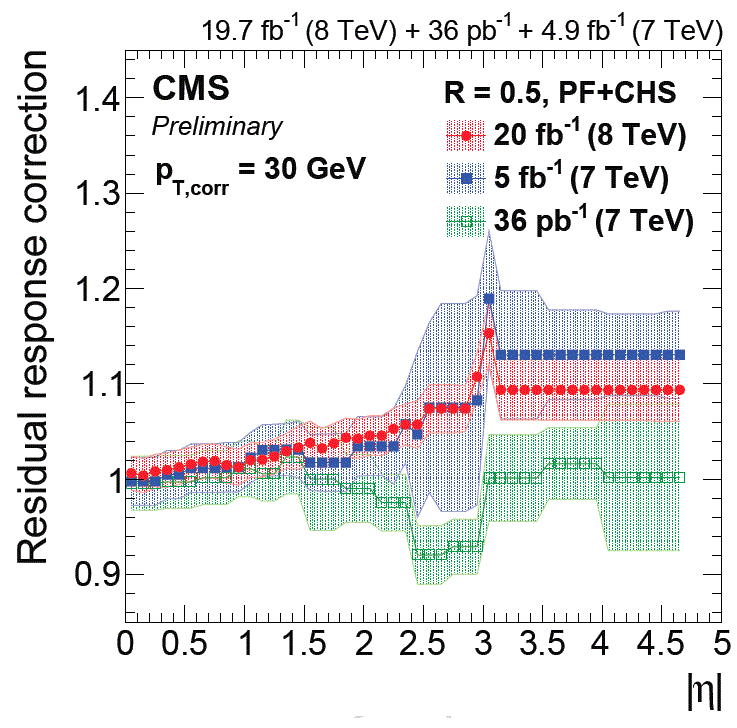
\includegraphics[width= 0.45\textwidth]{figures/staterror_jec_luminosity_pp.png}
\caption{Residual jet energy scale correction and its uncertainty as a function of
$\eta$ derived from different pp data sets at \roots\ = 7 and 8 TeV.}
\label{fig:jetJES}
\end{center}
\end{figure}

\clearpage